\begin{name}
	{\tenchude}
	{TOÁN 11}
	{LỚP TOÁN THẦY PHÁT}
	{Thời gian: 90 phút - Không kể thời gian phát đề}
\end{name}
\setcounter{ex}{0}\setcounter{bt}{0}
\noindent{\bf\fontfamily{qag}\selectfont\color{violet}A. PHẦN TRẮC NGHIỆM}
\Opensolutionfile{ans}[ans/ans-1-GK1-KNTT-De17-NH23-24]
%%==========Câu 1
\begin{ex}%[1K1Y1-1]
Số đo bằng độ của cung lượng giác $\dfrac{\pi}{12}$ là
\choice
{$\left(\dfrac{75}{2}\right)^{\circ}$}
{$45^{\circ}$}
{$-345^{\circ}$}
{\True $15^{\circ}$}
\loigiai{
	Ta có $\dfrac{\pi}{12}=\dfrac{\pi}{12} \cdot\left(\dfrac{180}{\pi}\right)^o=15^{\circ}.$
}
	\end{ex}
%%%Câu 2
\begin{ex}%[1K1Y1-1] 
Đổi $80^{\circ}$ sang radian
	\choice
{\True $\dfrac{4 \pi}{9}$}
{$\dfrac{2 \pi}{9}$}
{$\dfrac{\pi}{9}$}
{$\dfrac{5 \pi}{9}$}
\loigiai{
 Ta có : $80^{\circ}=80 \cdot \dfrac{\pi}{180}=\dfrac{4 \pi}{9}$.
}
\end{ex}
%%%Câu 3
\begin{ex}%[1K1Y1-3] 
Cung tròn bán kính bằng $8$ cm có số đo $3$ rad có độ dài là
	\choice
	{$\dfrac{8}{3}$ cm}
	{$\dfrac{3}{11}$ cm}
	{$11$ cm}
	{\True $24$ cm}
	\loigiai{
		Độ dài cung tròn $l=R\alpha=8\cdot 3=24$ cm.
	}
\end{ex}
	
%%==========Câu 4
\begin{ex}%[1K1Y1-6]
	Cho góc $\alpha$ thỏa mãn $\sin \alpha=\dfrac{4}{5}$ và $\dfrac{\pi}{2}<\alpha<\pi$. Tính $P=\dfrac{1}{1+\tan^2\alpha}$
	\choice
	{$P=-\dfrac{3}{5}$}
	{$P=\dfrac{3}{5}$}
	{$P=-\dfrac{9}{25}$}
	{\True $P=\dfrac{9}{25}$}
	\loigiai{
Ta có $\cos^2 x=1-\sin^2x=1-\left(\dfrac{4}{5}\right)^2=\dfrac{9}{25}$ nên $1+\tan^2x=\dfrac{1}{\cos^2x}=\dfrac{25}{9}$.\\
Do đó $P=\dfrac{1}{1+\tan^2x}=\dfrac{9}{25}$.
}
\end{ex}
%%%%Câu 5
\begin{ex}%[1K1B1-6]
Cho $\sin a=\dfrac{1}{3}$. Tính $P=\dfrac{3 \cot a+2 \tan a}{\cot a+\tan a}$
\choice
{$P=\dfrac{9}{26}$}
{\True $P=\dfrac{26}{9}$}
{$P=-6$}
{$P=6$}
\loigiai{
Ta có 
\[
P=\dfrac{3 \cot a+2 \tan a}{\cot a+\tan a}=\dfrac{3 \cot ^2 a+2}{\cot ^2 a+1}=\dfrac{3\left(\dfrac{1}{\sin ^2 a}-1\right)+2}{\dfrac{1}{\sin ^2 a}-1+1}=\dfrac{3 \dfrac{1}{\sin ^2 a}-1}{\dfrac{1}{\sin ^2 a}}=\dfrac{26}{9}
\]
}
\end{ex}
%%%%Câu 6
\begin{ex}%[1K1Y2-1]
Trong các công thức sau, công thức nào đúng?
\choice
{$\cos (a-b)=\cos a \cdot \cos b-\sin a \cdot \sin b$}
{\True $\cos (a-b)=\cos a \cdot \cos b+\sin a \cdot \sin b$}
{$\sin (a+b)=\sin a \cdot \cos b-\cos a \cdot \sin b$}
{$\sin (a-b)=\sin a \cdot \cos b+\cos a \cdot \sin b$}
\loigiai{
}
\end{ex}
%%%%Câu 7
\begin{ex}%[1T1Y3-2]
Trong các công thức sau, công thức nào \textbf{sai}?
\choice
{$\cos 2 a=\cos ^2 a-\sin ^2 a$}
{\True $\cos 2 a=\cos ^2 a+\sin ^2 a$}
{$\cos 2 a=2 \cos ^2 a-1$}
{$\cos 2 a=1-2 \sin ^2 a$}
\loigiai{

}
\end{ex}
%%%%Câu 8
\begin{ex}%[1K1Y2-2]
Cho $\cos 2 \alpha=\dfrac{1}{2}$. Tính giá trị biểu thức $P=5 \sin ^2 \alpha-4 \cos ^2 \alpha$.
\choice
{$\dfrac{7}{4}$}
{$-\dfrac{5}{8}$}
{\True $-\dfrac{7}{4}$}
{$\dfrac{1}{8}$}
 \loigiai{
  	$$
\begin{aligned}
	P=5 \sin ^2 \alpha-4 \cos ^2 \alpha & =5\left(\frac{1-\cos 2 \alpha}{2}\right)-4\left(\frac{1+\cos 2 \alpha}{2}\right) \\
	& =\frac{1}{2}-\frac{9}{2} \cos 2 \alpha=\frac{1}{2}-\frac{9}{2} \cdot \frac{1}{2}=-\frac{7}{4} .
\end{aligned}
$$
}
\end{ex}
%%%%%câu 9
\begin{ex}%[1K1B2-1]
Cho hai góc $\alpha, \beta$ thỏa mãn $\sin \alpha=\dfrac{5}{13},\left(\dfrac{\pi}{2}<\alpha<\pi\right)$ và $\cos \beta=\dfrac{3}{5},\left(0<\beta<\dfrac{\pi}{2}\right)$. Tính giá trị đúng của $\cos (\alpha-\beta)$.
\choice
{$\dfrac{16}{65}$}
{\True $-\dfrac{16}{65}$}
{$\dfrac{18}{65}$}
{$-\dfrac{18}{65}$}
\loigiai{
Ta có\\
$\sin \alpha=\dfrac{5}{13},\left(\dfrac{\pi}{2}<\alpha<\pi\right)$ nên $\cos \alpha=-\sqrt{1-\sin ^2 \alpha}=-\sqrt{1-\left(\dfrac{5}{13}\right)^2}=-\dfrac{12}{13}$.\\
$\cos \beta=\dfrac{3}{5},\left(0<\beta<\dfrac{\pi}{2}\right)$ nên $\sin \beta=\sqrt{1-\cos ^2 \beta}=\sqrt{1-\left(\dfrac{3}{5}\right)^2}=\dfrac{4}{5}$.\\
Do đó $\cos (\alpha-\beta)=\cos \alpha \cos \beta+\sin \alpha \sin \beta=-\dfrac{12}{13} \cdot \dfrac{3}{5}+\dfrac{5}{13} \cdot \dfrac{4}{5}=-\dfrac{16}{65}$.
}
\end{ex}
%%%%Câu 10
\begin{ex}%[1K1K2-3]
Rút gọn biểu thức: $\dfrac{\sin a+\sin 3 a+\sin 5 a}{\cos a+\cos 3 a+\cos 5 a}$.
\choice
{\True $\tan 3a$}
{$\tan a$}
{$2 \tan 3 a$}
{$\cot 3 a$}
 \loigiai{
 	Ta có
	$$
	\begin{aligned}
		 \dfrac{\sin a+\sin 3 a+\sin 5 a}{\cos a+\cos 3 a+\cos 5 a}&=\dfrac{\sin a+\sin 5 a+\sin 3 a}{\cos a+\cos 5 a+\cos 3 a}=\dfrac{2 \sin 3 a \cdot \cos a+\sin 3 a}{2 \cos 3 a \cdot \cos a+\cos 3 a} \\
		&= \dfrac{\sin 3 a \cdot(2 \cos a+1)}{\cos 3 a \cdot(2 \cos a+1)}=\tan 3 a .
	\end{aligned}
	$$
}
\end{ex}
%%%%Câu 11
\begin{ex}%[1K1Y3-1]
Xét bốn mệnh đề sau:
\begin{enumerate}
	\item [(1)] Hàm số $y=\sin x$ có tập xác định là $\mathbb{R}$.
	\item [(2)] Hàm số $y=\cos x$ có tập xác định là $\mathbb{R}$.
	\item [(3)] Hàm số $y=\tan x$ có tập xác định là $D=\mathbb{R} \backslash\left\{\dfrac{\pi}{2}+k \pi \mid k \in \mathbb{Z}\right\}$.
	\item [(4)] Hàm số $y=\cot x$ có tập xác định là $D=\mathbb{R} \backslash\left\{k \dfrac{\pi}{2} \mid k \in \mathbb{Z}\right\}$.
\end{enumerate}
Số mệnh đề đúng là 
\choice
{\True $3$}
{$2$}
{$1$}
{$4$}
\loigiai{
Các mệnh đề đúng là:
\begin{enumerate}[1)]
	\item  Hàm số $y=\sin x$ có tập xác định là $\mathbb{R}$.
\item (2) Hàm số $y=\cos x$ có tập xác định là $\mathbb{R}$.
\item (3) Hàm số $y=\tan x$ có tập xác định là $D=\mathbb{R} \backslash\left\{\frac{\pi}{2}+k \pi \mid k \in \mathbb{Z}\right\}$.
\end{enumerate}
}
\end{ex}
%%%%Câu 12
\begin{ex}%[1K1Y3-4]
Chu kỳ tuần hoàn của hàm số $y=\tan x$ là
\choice
{$k \pi, (k \in \mathbb{Z})$}
{\True $\pi$}
{$\dfrac{\pi}{3}$}
{$3 \pi$}
\loigiai{
	Hàm số $y=\tan x$ tuần hoàn với chu kỳ là $\pi$.
}
\end{ex}
%%%Câu 13
\begin{ex}%[1K1B3-4]
Tìm chu kì của hàm số $f(x)=\sin \dfrac{x}{2}+2 \cos \dfrac{3 x}{2}$.
\choice
{$5 \pi$}
{$\dfrac{\pi}{2}$}
{\True $4 \pi$}
{$2 \pi$}
\loigiai{
Chu kỳ của $\sin \dfrac{x}{2}$ là $T_1=\dfrac{2 \pi}{\left|\dfrac{1}{2}\right|}=4 \pi$ và chu kỳ của $\cos \dfrac{3 x}{2}$ là $T_2=\dfrac{2 \pi}{\left|\dfrac{3}{2}\right|}=\dfrac{4 \pi}{3}$.\\
Chu kì của hàm ban đầu là bội chung nhỏ nhất của hai chu kì $T_1$ và $T_2$ vừa tìm được ở trên. Do đó chu kì của hàm ban đầu $T=4 \pi$.  
}
\end{ex}
%%%%Câu 14
\begin{ex}%[1K1B3-3]
Xét tính chẵn lẻ của hàm số $y=\dfrac{\sin 2 x}{2 \cos x-3}$ thì $y=f(x)$ là
\choice
{Hàm số chẵn}
{\True Hàm số lẻ}
{Không chẵn không lẻ}
{Vừa chẵn vừa lẻ}
 \loigiai{
 Tập xác định $\mathscr{D}=\mathbb{R}$.\\
 Ta có $\forall x \in \mathscr{D} \Rightarrow-x \in \mathscr{D}$.\\
 $f(-x)=\dfrac{\sin (-2 x)}{2 \cos (-x)-3}=\dfrac{-\sin 2 x}{2 \cos x-3}=-f(x)$.\\
 Vậy hàm số đã cho là hàm số lẻ.}
\end{ex}
%%%%Câu 15
\begin{ex}%[1K1B3-5]
Giá trị nhỏ nhất của hàm số $y=2 \cos ^2 x-\sin 2 x+5$.
\choice
{$\sqrt{2}$}
{$-\sqrt{2}$}
{\True $6-\sqrt{2}$}
{$6+\sqrt{2}$}
\loigiai{
Ta có $y=2 \cos ^2 x-\sin 2 x+5=\cos 2 x-\sin 2 x+6=\sqrt{2} \cos \left(2 x+\dfrac{\pi}{4}\right)+6$.\\
	Do $-\sqrt{2} \leq \sqrt{2} \cos \left(2 x+\dfrac{\pi}{4}\right) \leq \sqrt{2}$ nên $-\sqrt{2}+6 \leq \sqrt{2} \cos \left(2 x+\dfrac{\pi}{4}\right)+6 \leq \sqrt{2}+6$.\\
	Vậy giá trị nhỏ nhất của hàm số $y=2 \cos ^2 x-\sin 2 x+5$ là $6-\sqrt{2}$.
}
\end{ex}
%%%Câu 16
\begin{ex}%[1K1Y4-3]
Cho $x=\dfrac{\pi}{2}+k 2 \pi, k \in \mathbb{Z}$ là nghiệm của phương trình nào sau đây
\choice
{$\sin x=0$}
{\True $\sin x=1$}
{$\sin x=-1$}
{$\cos x=1$}
 \loigiai{
	$$
	\sin x=1 \Leftrightarrow x=\frac{\pi}{2}+k 2 \pi, k \in \mathbb{Z}.
	$$
}
\end{ex}
%%%Câu 17
\begin{ex}%[1K1Y4-3]
Trong các phương trình sau, phương trình nào vô nghiệm?
\choice 
{$\sin x=\dfrac{1}{2}$}
{\True $\sin x=\dfrac{5}{3}$}
{$\tan x=-2023$}
{$\cos x=\dfrac{3}{5}$}
 \loigiai{
Phương trình $\sin x=a$ có nghiệm khi $|a| \leq 1$.
}
\end{ex}
%%%%Vâu 18
\begin{ex}%[1K1Y4-3]
Phương trình $\sin x=m-1$ có nghiệm khi $m$ là
\choice
{$-1 \leq m \leq 1$}
{\True $0 \leq m \leq 2$}
{$m \leq 0$}
{$-1 \leq m \leq 0$}
\loigiai{
Phương trình $\sin x=m-1$ có nghiệm khi $-1 \leq m-1 \leq 1 \Leftrightarrow 0 \leq m \leq 2$
}
\end{ex}
%%%Câu 19
\begin{ex}%[1K1B4-3]
Phương trình $1+2 \sin x \cos x=0$ có nghiệm là
\choice
{$x=\dfrac{\pi}{2}+k 2 \pi$}
{\True $x=-\dfrac{\pi}{4}+k \pi$}
{$x=-\dfrac{\pi}{3}+k 2 \pi$}
{$x=-\dfrac{\pi}{3}+k \pi$}
 \loigiai{
Phương trình: $1+2 \sin x \cos x=0 \Leftrightarrow \sin 2 x=-1 \Leftrightarrow 2 x=-\dfrac{\pi}{2}+k 2 \pi \Leftrightarrow x=-\dfrac{\pi}{4}+k \pi$
}
\end{ex}
%%%Câu 20
\begin{ex}%[1K1Y4-A]
Phương trình $(2 \cos x+1)(\cos 2 x-\sqrt{3})=0$ có nghiệm là
\choice
{$x=\dfrac{\pi}{2}+k 2 \pi$}
{\True $x= \pm \dfrac{2 \pi}{3}+k 2 \pi$}
{$x= \pm \dfrac{\pi}{4}+k 2 \pi$}
{$x= \pm \dfrac{\pi}{6}+k 2 \pi$}
  \loigiai{
Phương trình 
\allowdisplaybreaks
\begin{eqnarray*}
(2 \cos x+1)(\cos 2 x-\sqrt{3})=0 \Leftrightarrow \hoac{&\cos x=-\dfrac{1}{2} \\ &\cos 2 x=\sqrt{3} \quad (\text{Vô Nghiệm})}
\end{eqnarray*}
Với $	\cos x=-\dfrac{1}{2} \Leftrightarrow x= \pm \dfrac{2 \pi}{3}+k 2 \pi
	$}
\end{ex}
%%%Câu 21
\begin{ex}%[1K1B4-A]
\textit{(Bảng số liệu sau dùng cho câu 21-24)}
Quãng đường (km) các cầu thủ (không tính thủ môn) chạy trong một trận bóng đá tại giải ngoại hạng Anh được cho trong bảng thống kê sau:
	\begin{center}
		\begin{tabular}{|c|c|c|c|c|c|}
			\hline Quãng đường & {$[2 ; 4)$} & {$[4 ; 6)$} & {$[6 ; 8)$} & {$[8 ; 10)$} & {$[10 ; 12)$} \\
			\hline Số cầu thủ & 2 & 5 & 6 & 9 & 3 \\
			\hline
		\end{tabular}
	\end{center}
	Tính quãng đường trung bình một cầu thủ chạy trong trận đấu này.
	\choice{$7{,}02$}{\True $7{,}48$}{$5{,}23$}{$8{,}36$}
		\loigiai{
			Tổng số cầu thủ là $n=2+5+6+9+3=25$.\\
			Quãng đường trung bình một cầu thủ chạy trong trận đấu này là
			$$\overline{x}=\dfrac{2\cdot 3+5\cdot 5+6\cdot 7+9\cdot 9+3\cdot 11}{25}=7{,}48~(\mathrm{km}).$$ 
		}
\end{ex}
%%%%Câu 22
\begin{ex}%[1K2Y5-2]
	Tìm trung vị của mẫu số liệu.
	\choice{\True $7{,}83$}{$7{,}48$}{$6{,}23$}{$3{,}56$}
		\loigiai{
			Cỡ mẫu $n = 2 + 5 + 6 + 9 + 3 = 25$.\\
			Gọi $x_1, x_2, \ldots, x_{25}$ là quãng đường chạy của $25$ cầu thủ và giả sử dãy này đã được sắp xếp theo thứ tự không giảm. Khi đó, trung vị là $x_{13}$, mà $x_{13}$ thuộc nhóm $[6; 8)$ nên nhóm này chứa trung vị. Do đó, trung vị là
			$$	M_e=6+\dfrac{\dfrac{25}{2}-(2+5)}{6}\cdot (8-6) \approx 7{,}83.	$$			
		}
\end{ex}
%%%Câu 23
\begin{ex}%[1K2Y5-2]
Tìm $a$ sao cho có $25 \%$ số cầu thủ tham gia trận đấu chạy ít nhất $a~(\mathrm{km})$.
\choice
{\True $9{,}28$}
{$7{,}48$}
{$12{,}23$}
{$13{,}56$}
		\loigiai{
			Số $a$ thỏa mãn có $25 \%$ số cầu thủ tham gia trận đấu chạy ít nhất $a$ (km).\\
			Do đó, $a$ chính là tứ phân vị thứ ba của mẫu số liệu trên.\\
			Cỡ mẫu $n=25$.\\
			Gọi $x_1, x_2 \ldots, x_{25}$ là quãng đường chạy của $25$ cầu thủ và giả sử dãy này đã được sắp xếp theo thứ tự không giảm. Khi đó tứ phân vị thứ ba là $\dfrac{x_{19}+x_{20}}{2}$.\\ Do $x_{19}, x_{20}$ đều thuộc nhóm $[8 ; 10)$ nên nhóm này chứa tứ phân vị thứ ba.\\ Do đó $a=Q_3=8+\dfrac{\dfrac{3.25}{4}-(2+5+6)}{9} \cdot(10-8) \approx 9{,}28$. 
		}
\end{ex}
%%%%Câu 24
\begin{ex}%[1K2B5-3]
Tính mốt của mẫu số liệu thu được.
\choice{$9{,}28$}{$7{,}48$}{\True $8{,}67$}{$13{,}56$}
		\loigiai{
			Tần số lớn nhất là $9$ nên nhóm chứa mốt là $[8; 10)$.\\
			Mốt là $M_o=8+\dfrac{(9-6)}{(9-6)+(9-3)} \cdot 2 \approx 8{,}67$.\\
}
\end{ex}
%%%%%Câu 25
\begin{ex}%[1K2B5-4]
Cho dãy số $\left(u_n\right)$ biết $u_n=\dfrac{4 n+5}{n+1}$. Mệnh đề nào sau đây đúng?
\choice
{Dãy số bị chặn trên}
{Dãy số bị chặn dưới}
{\True Dãy số bị chặn}
{Không bị chặn}
\loigiai{
Ta có $u_n=\dfrac{4 n+5}{n+1}>0, \forall n \in \mathbb{N}^*$. Khi đó
$$
u_n=\dfrac{4 n+5}{n+1}=\dfrac{4(n+1)+1}{n+1}=4+\dfrac{1}{n+1} \leq 4+\dfrac{1}{2}=\dfrac{9}{2} \Rightarrow u_n \leq \dfrac{9}{2}, \forall n \in \mathbb{N}^*
$$
Suy ra $0<u_n \leq \dfrac{9}{2}, \forall n \in \mathbb{N}^*$.\\
Vậy dãy số $\left(u_n\right)$ bị chặn.
}
\end{ex}
%%%%Câu 26
\begin{ex}%[1K2Y6-3]
Cho cấp số cộng có số hạng đầu $u_1=-\dfrac{1}{2}$, công sai $d=\dfrac{1}{2}$. Năm số hạng liên tiếp đầu tiên của cấp số này là
\choice
{$-\dfrac{1}{2}; 0; 1; \dfrac{1}{2}; 1$}
{$-\dfrac{1}{2}; 0; \dfrac{1}{2}; 0; \dfrac{1}{2}$}
{$\dfrac{1}{2}; 1; \dfrac{3}{2}; 2; \dfrac{5}{2}$}
{\True $-\dfrac{1}{2}; 0; \dfrac{1}{2}; 1; \dfrac{3}{2}$}
 \loigiai{
Ta có $u_1=-\dfrac{1}{2}$ và $d=\dfrac{1}{2}$ nên  \[\heva{&u_1=-\dfrac{1}{2} \\ &u_2=u_1+d=0 \\ &u_3-u_2+d=\dfrac{1}{2} \\ &u_4=u_3+d=1 \\ &u_5=u_4+d=\dfrac{3}{2}}.\]
Vậy $5$ số hạng cần tìm là $-\dfrac{1}{2}; 0; \dfrac{1}{2}; 1; \dfrac{3}{2}$.
}
\end{ex}
%%%%Câu 27
\begin{ex}%[1K2Y6-3]
Cho cấp số cộng $\left(u_n\right)$ biết $u_1=2$ và công sai $d=3$. Tính $u_2$ bằng
\choice
{\True $5$}
{$6$}
{$7$}
{$8$}
\loigiai{
	Ta có: $u_2=u_1+d=2+3=5$.
}
\end{ex}
%%%Câu 28
\begin{ex}%[1K2B6-1]
Cho cấp số cộng $\left(u_n\right)$ thỏa mãn $\heva{&u_4=10 \\& u_4+u_6=26}$ có công sai là
\choice
{$d=-3$}
{\True $d=3$}
{$d=5$}
{$d=6$}
\loigiai{
Ta có: $\heva{&u_4=10 \\& u_4+u_6=26} \Leftrightarrow\heva{&u_1+3 d=10 \\& 2 u_1+8 d=26} \Leftrightarrow\heva{&u_1=1 \\& d=3.}$
\\Vậy công sai $d=3$.
}
\end{ex}
%%%%Câu 29
\begin{ex}%[1K2B6-1]
Cho cấp số cộng $\left(u_n\right)$ biết $u_1=1$ và $u_4=10$. Công sai $d$ bằng
\choice
{$-2$}
{$1$}
{\True $3$}
{$-4$}
\loigiai{
Ta có $u_4=u_1+3 d=1+3 d=10 \Leftrightarrow d=3$.
}
\end{ex}
%%%%Câu 30
\begin{ex}%[1K2B6-5]
Tính tổng $K=15+20+25+\ldots+7510$.
\choice
{$5\,634\,750$ }
{$5\,643\,705$}
{$5\,643\,250$}
{\True $5\,643\,750$}
 \loigiai{	Ta thấy các số hạng của tổng $K$ tạo thành một cấp số cộng với số hạng đầu $u_1=15$ và công sai $d=5$.\\
	Giả sử tổng trên có $n$ số hạng thì 
	\[u_n=7510
	\Leftrightarrow u_1+(n-1) d=7\,510 \Leftrightarrow 15+(n-1) 5=7\,510 \Leftrightarrow n=1\,500.\]
Vậy $K=S_{1\,500}=\dfrac{1\,500(15+7\,510)}{2}=5\,643\,750$.}
\end{ex}
%%%%Câu 31
\begin{ex}%[1K2Y7-1]
Cho cấp số nhân $\left(u_n\right)$ biết $u_1=3$ và công bội $q=2$. Tính $u_4$ bằng
\choice
{$9$}
{$16$}
{\True $24$}
{$48$}
 \loigiai{
	Ta có $u_4=u_1 \cdot q^3=3 \cdot 2^3=24$.
}
\end{ex}
%%%%Câu 32
\begin{ex}%[1K2Y7-1]
Cho cấp số nhân $\left(u_n\right)$ biết $u_1=5$ và $u_2=-20$. Công bội $q$ bằng
\choice
{$-2$}
{$4$}
{$3$}
{\True $-4$}
\loigiai{	Ta có $q=\dfrac{u_2}{u_1}=\dfrac{-20}{5}=-4$.
}
\end{ex}
%%%%Câu 33
\begin{ex}%[1K2Y7-3]
Cho cấp số nhân: $1 ; 2 ; 4 ; 8 ; \ldots$ Số hạng thứ năm là
\choice
{$10$}
{\True $16$}
{$12$}
{$32$}
\loigiai{	Ta có công bội $q=\dfrac{u_2}{u_1}=\dfrac{2}{1}=2$.\\
	Suy ra $u_5=u_4 \cdot q=8.2=16$.
}
\end{ex}
%%%%Câu 34
\begin{ex}%[1K2B7-5]
Cho cấp số nhân $\left(u_n\right)$ biết $u_1=5$ và công bội $q=2$. Tính tổng của $10$ số hạng đầu tiên $S_{10}$
\choice
{$4225$}
{$4115$}
{$5225$}
{\True $5115$}
 \loigiai{
Ta có: $S_{10}=u_1 \cdot \dfrac{1-q^{10}}{1-q}=5 \cdot \dfrac{1-2^{10}}{1-2}=5115$.
}
\end{ex}
%%%%Câu 35
\begin{ex}%[1K2B7-1]
Cho cấp số nhân $\left(u_n\right)$ biết $\heva{&u_4+u_6=540 \\& u_1+u_3=20}$. Công bội $q$ bằng
\choice
{$6$}
{$27$}
{$2$}
{\True$3$}
 \loigiai{
	Ta có:
	\allowdisplaybreaks
	\begin{eqnarray*}
\heva{&u_4+u_6=540 \\& u_1+u_3=20} \Leftrightarrow\heva{&u_1 q^3 \cdot\left(1+q^2\right)=540 \\& u_1\left(1+q^2\right)=20} \Leftrightarrow\heva{&q^3=27 \\& u_1\left(1+q^2\right)=20} \Leftrightarrow\heva{&q=3 \\& u_1=2.}
\end{eqnarray*}
}
\end{ex}


\Closesolutionfile{ans}
% \inputans{10}{ans/ans-1-GK1-KNTT-De17-NH23-24}
\noindent{\bf\fontfamily{qag}\selectfont\color{violet}B. PHẦN TỰ LUẬN}
\setcounter{bt}{0}
%%==========Bài 1
 \begin{bt}%[1K1Y1-6]
Cho $\sin \alpha=\dfrac{3}{5}$ và $\dfrac{\pi}{2}<\alpha<\pi$. Tính giá trị của $\cos \alpha$ ?
\loigiai{
 Ta có 
 \[\sin ^2 \alpha+\cos ^2 \alpha=1 \Rightarrow \cos ^2 \alpha=1-\sin ^2 \alpha=1-\dfrac{9}{25}=\dfrac{16}{25} \Leftrightarrow\hoac{&\cos \alpha=\frac{4}{5} \\& \cos \alpha=-\dfrac{4}{5}.}\] 
 Vì $\dfrac{\pi}{2}<\alpha<\pi$ nên $\cos \alpha<0$, do đó $\cos \alpha=-\dfrac{4}{5}$.
} 
 \end{bt}
%%%%%Bài 37
\begin{bt}%[1K2B6-6]
Trong dịp nghỉ lễ 02/9 gia đình anh An cần thuê một xe Taxi để di chuyển từ thủ đô Hà Nội về thăm quê tại TP Bắc Giang. Biết giá của kilômét đầu tiên là $10.000$ đồng, kể từ kilômét thứ 2 giá của mỗi kilômét tăng thêm $500$ đồng so với giá của kilômét trước đó. Biết quãng đường Taxi di chuyển từ thủ đô Hà Nội về TP Bắc Giang là $80$ km. Hỏi gia đình anh An phải trả bao nhiêu tiền cho chuyến Taxi đó?
\loigiai{
Số tiền ở từng kilômet lập thành một cấp số cộng.\\
Số hạng đầu tiên là $u_1=10.000$, công sai $d=500$.\\
Cấp số cộng có $80$ số hạng.\\
Tổng số tiền là $S_{80}=80.10000+\dfrac{79.80 .500}{2}=2.380 .000$ đồng.
}
\end{bt}
%%%%Bài 38
\begin{bt}%[1D1T5-6]
	\immini{
		Một chiếc guồng nước có dạng hình tròn bán kính $2{,}5$ m; trục của nó đặt cách mặt nước $2$ m (hình bên). Khi guồng quay đều, khoảng cách $h$ (m) tính từ một chiếc gầu tại điểm $A$ trên guồng đến mặt nước là $h=|y|$ trong đó $$y=2+2{,}5\sin 2\pi\left(x-\dfrac{1}{4}\right)$$ với $x$ là thời gian quay của guồng ($x\ge 0$), tính bằng phút; ta quy ước rằng $y>0$ khi gầu ở trên mặt nước và $y<0$ khi gầu ở dưới mạt nước
		\begin{enumerate}
			\item Khi nào chiếc gầu ở vị trí cao nhất? Thấp nhất?
			\item Chiếc gầu cách mặt nước $2$ mét lần đầu tiên khi nào?
		\end{enumerate}
	}
	{
		\begin{tikzpicture}[>=stealth,line join=round,line cap=round,font=\footnotesize,scale=1]
			\def\r{2.5}
			\coordinate[label=above:$O$] (O) at (0,0);
			\draw[name path=(C)] (O) circle (\r);
			\coordinate (M) at (0,-2);
			\path 
			(O)++(45:\r)coordinate(A)node[above right]{$A$}
			(-3,-2)coordinate(B)
			(3,-2)coordinate(C)
			($(B)!(A)!(C)$)coordinate(H)
			;
			\draw[dashed] (A)--(H)node[midway,right]{$h$ m}
			(B)--(C)
			;
			\draw[<->](O)--(A)node[midway,left]{$2{,}5$ m};
			\draw[<->](O)--(M)node[midway,right]{$2$ m};
			\draw[->] (A) arc (45:60:2.5);
		\end{tikzpicture}
	}
	\loigiai 
	{
		\begin{enumerate}
			\item Với mọi $x\in \mathbb{R}$, ta có
			\allowdisplaybreaks
			\begin{eqnarray*}
				-1\le \sin 2\pi\left(x-\dfrac{1}{4}\right)\le 1&\Leftrightarrow&-2{,}5\le 2{,}5\sin 2\pi\left(x-\dfrac{1}{4}\right)\le 2{,}5\\
				&\Leftrightarrow&-0{,}5\le 2+2{,5}\sin 2\pi\left(x-\dfrac{1}{4}\right)\le 4{,}5.
			\end{eqnarray*}
			Suy ra, gầu ở vị trí cao nhất khi 
			$$\sin 2\pi\left(x-\dfrac{1}{4}\right)=1\Leftrightarrow 2x\left(x-\dfrac{1}{4}\right)=\dfrac{\pi}{2}+k2\pi\Leftrightarrow x=\dfrac{1}{2}+k, \,(k\in\mathbb{Z}).$$
			Vậy gầu ở vị trí cao nhất tại các thời điểm $\dfrac{1}{2}$, $\dfrac{3}{2}$, $\dfrac{5}{2}$,$\ldots$ phút.\\
			Tương tự, gầu ở vị trí thấp nhất khi 
			$$\sin 2\pi\left(x-\dfrac{1}{4}\right)=-1\Leftrightarrow 2x\left(x-\dfrac{1}{4}\right)=-\dfrac{\pi}{2}+k2\pi\Leftrightarrow xk, \,(k\in\mathbb{Z}).$$
			Vậy gầu ở vị trí thấp nhất tại các thời điểm $0$, $1$, $2$,$\ldots$ phút.
			\item Gầu các mặt nước $2$ m nên 
			\allowdisplaybreaks
			\begin{eqnarray*}
				2+2{,}5\sin 2\pi\left(x-\dfrac{1}{2}\right)=2&\Leftrightarrow&\sin 2\pi\left(x-\dfrac{1}{2}\right)=0\\
				&\Leftrightarrow&2\pi\left(x-\dfrac{1}{4}\right)=k\pi\\
				&\Leftrightarrow&x=\dfrac{1}{4}+\dfrac{k}{2},\,(k\in\mathbb{Z}).
			\end{eqnarray*}
			Vậy chiếc gầu cách mặt nước $2$ m lần đầu tiên tại thời điểm $x=\dfrac{1}{4}$ phút.
		\end{enumerate}		
	}
\end{bt}
%%%%Bài 39
\begin{bt}%[1K2B7-7]
		Từ tờ giấy, cắt một hình tròn bán kính $R$ (cm). Tiếp theo, cắt hai hình tròn bán kính $\dfrac{R}{2}$ rồi chồng lên hình tròn đầu tiên . Tiếp theo, cắt bốn hình tròn bán  kính $\dfrac{R}{4}$ 
		rồi chồng lên các hình trước. Cứ thế tiếp tục mãi. Tính tổng diện tích của các hình tròn.
	\begin{center}
		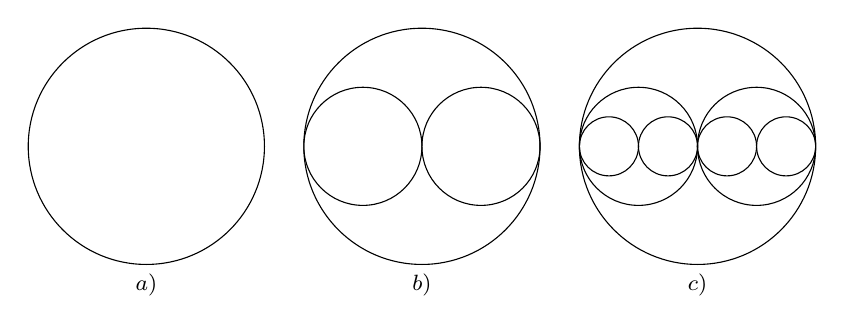
\begin{tikzpicture}[>=stealth,line join=round,line cap=round,font=\footnotesize,scale=1,declare function={r=1.5;}]
			\begin{scope}
				\draw (0,0)circle(r);
				\path (0,-r) node[below]{$a)$};
			\end{scope}
			\begin{scope}[xshift={3.5cm}]
				\draw(0,0)circle(r);
				\draw (r/2,0)circle(r/2);
				\draw(-r/2,0)circle(r/2);
				\path (0,-r) node[below]{$b)$};
			\end{scope}
			\begin{scope}[xshift={7cm}]
				\draw (0,0)circle(r);
				\draw (r/2,0)circle(r/2);
				\draw (-r/2,0)circle(r/2);
				\foreach \i in {0,1,2,3}
				\draw[shift={(r/2*\i,0)}] (-3*r/4,0)circle(r/4);
				\path (0,-r) node[below]{$c)$};
			\end{scope}
			% \path (current bounding box.south) node[below]{Hình $3$};
		\end{tikzpicture}
	\end{center}
	\loigiai{
		Diện tích của các hình tròn trong các lần cắt là
		\begin{enumerate}
			\item Lần thứ 1: $S_1=\pi R^2$.
			\item  Lần thứ 2: $S_2=2\cdot \pi \left(\dfrac{R}{2}\right)^2= \dfrac{\pi R^2}{2}$.
			\item  Lần thứ 3: $S_2=4\cdot \pi \left(\dfrac{R}{4}\right)^2= \dfrac{\pi R^2}{2^2}$.	
			\item Lần thứ $n$: $S_n= \dfrac{\pi R^2}{2^{n-1}}$.
		\end{enumerate}
		Do đó  diện tích các hình tròn lập thành một cấp số nhân lùi vô hạn có số hạng đầu $S_1=\pi R^2$ và công bội $q=\dfrac{1}{2}$ nên tổng diện tích các hình tròn là 
		\[ S_1+S_2+\cdots=\dfrac{\pi R^2}{1-\dfrac{1}{2}}=2\pi R^2. \]
	}
\end{bt}

